
\begin{figure}[H]
  \centering
  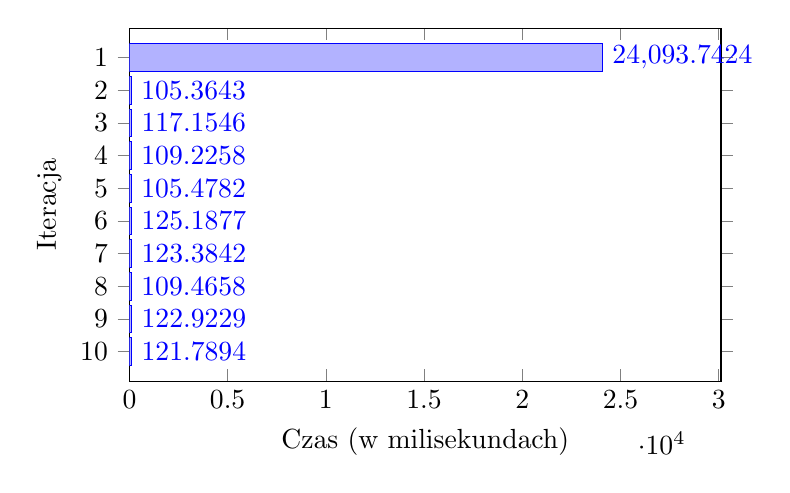
\begin{tikzpicture}
  
    \begin{axis} [
      xbar = .05cm,
      nodes near coords,
      nodes near coords style={
        /pgf/number format/precision=4,
      },
      xmin = 0,
      ytick = data,
      enlarge x limits = {value = .25, upper},
      symbolic y coords = {10,9,8,7,6,5,4,3,2,1},
      xlabel=Czas (w milisekundach),
      ylabel=Iteracja,
      width=0.75\textwidth,
      height=0.5\textwidth
    ]
    
      \addplot coordinates {(24093.74239999056,1) (105.3643000125885,2) (117.15460002422333,3) (109.22579997777939,4) (105.47820001840591,5) (125.18769997358322,6) (123.38419997692108,7) (109.46579998731613,8) (122.9229000210762,9) (121.78940004110336,10)};
      
    \end{axis}
  
  \end{tikzpicture}
  \caption{Wynik testów przykładu 9 [\ref{lst:wydajnosc-przyklad-p-9}]}
  \label{fig:wynik-przyklad-8}
\end{figure}
